\documentclass[a4paper,14pt]{extarticle}

\usepackage[a4paper,top=20mm,bottom=20mm,left=30mm,right=10mm]{geometry}
\usepackage[T1,T2A]{fontenc}
\usepackage[utf8]{inputenc}
\usepackage[russian]{babel}
\usepackage{indentfirst}
\usepackage{titlesec}
\usepackage{graphicx}
\usepackage{verbatim}
\usepackage{fancyvrb}

\renewcommand{\baselinestretch}{1.3}
\titleformat{\section}{\normalsize\bfseries}{\thesection}{1em}{}
\titleformat{\subsection}{\normalsize\bfseries}{\thesection}{1em}{}
\setlength{\parindent}{12.5mm}

\begin{document}

  \newpage\thispagestyle{empty}
  \begin{center}
    \MakeUppercase{
      Министерство науки и высшего образования Российской Федерации\\
      Федеральное государственное бюджетное образовательное учреждение высшего образования\\
      <<Вятский Государственный Университет>>\\
    }
    Институт математики и информационных систем\\
    Факультет автоматики и вычислительной техники\\
    Кафедра электронных вычислительных машин
  \end{center}
  \vfill

  \begin{center}
    Отчет по лабораторной работе №5\\
    по дисциплине\\
    <<Управление данными>>\\
  \end{center}
  \vfill

  \noindent
  \begin{tabular}{ll}
    Выполнил студент гр. ИВТб-2301-05-00 \hspace{5mm} &
    \rule[-1mm]{25mm}{0.10mm}\,/Макаров С.А./\\
    
    Преподаватель & \rule[-1mm]{25mm}{0.10mm}\,/Клюкин В.Л./\\
  \end{tabular}

  \vfill
  \begin{center}
    Киров 2025
  \end{center}

  \newpage
  \section*{Цель}
  Цель лабораторной работы: познакомиться с библиотекой в Python для связывания приложения с БД, освоить на практике основы взаимодействия с БД под управлением PostgreSQL в приложении на Python.

  \section*{Задание}
  Создать приложение с графическим приложением на языке Python. Приложение должно использовать БД, разработанную в предыдущих лабораторных работах.

  Требования к интерфейсу:
  \begin{itemize}
    \item[--] Названия колонок, кнопок, объектов ввода/вывода на русском языке (Например, ‘Имя’, а не ‘Name’),
    \item[--] Запретить ввод отрицательных значений (Например, цена не может быть отрицательной),
    \item[--] Ввод данных для выборки должен быть регистронезависимый (используйте функции UPPER или LOWER),
    \item[--] Для ввода даты, по возможности, использовать календарь.
  \end{itemize}

  Для любой одной таблицы, которая содержит внешний ключ на другую таблицу, приложение должно выполнять следующие функции:
  \begin{itemize}
    \item[--] Выводить, удалять и изменять данные таблицы,
    \item[--] В случае ввода уже имеющихся данных выводить сообщение об этом пользователю без записи данных в таблицу,
    \item[--] Удалять при подтверждении (Например, ‘Вы действительно уверены?’ Да/Нет),
    \item[--] Выполнять фильтр (выборку) по значениям строк. (Например, «Дата с … по …» или «Имя содержит …»).
  \end{itemize}

  Требования к реализации:
  \begin{itemize}
    \item[--] При добавлении новой строки внешний ключ выбирается из списка значений родительской таблицы (например, если таблица «Чек» ссылается на таблицу «Товар», нужно вывести список не id товара, а его название),
    \item[--] Сохранение или удаление строки должно быть реализовано с помощью функции PL/pgSQL
    \item[--] Фильтрация значений при поиске должна производиться через запрос, а не в полученной коллекции
    \item[--] Разрешается использование любого фреймворка,
    \item[--] При разработке можно использовать шаблоны проектирования, связанные с работой с БД
  \end{itemize}

  \pagebreak
  \section*{Решение}
  \begin{figure}[h]
    \centering
    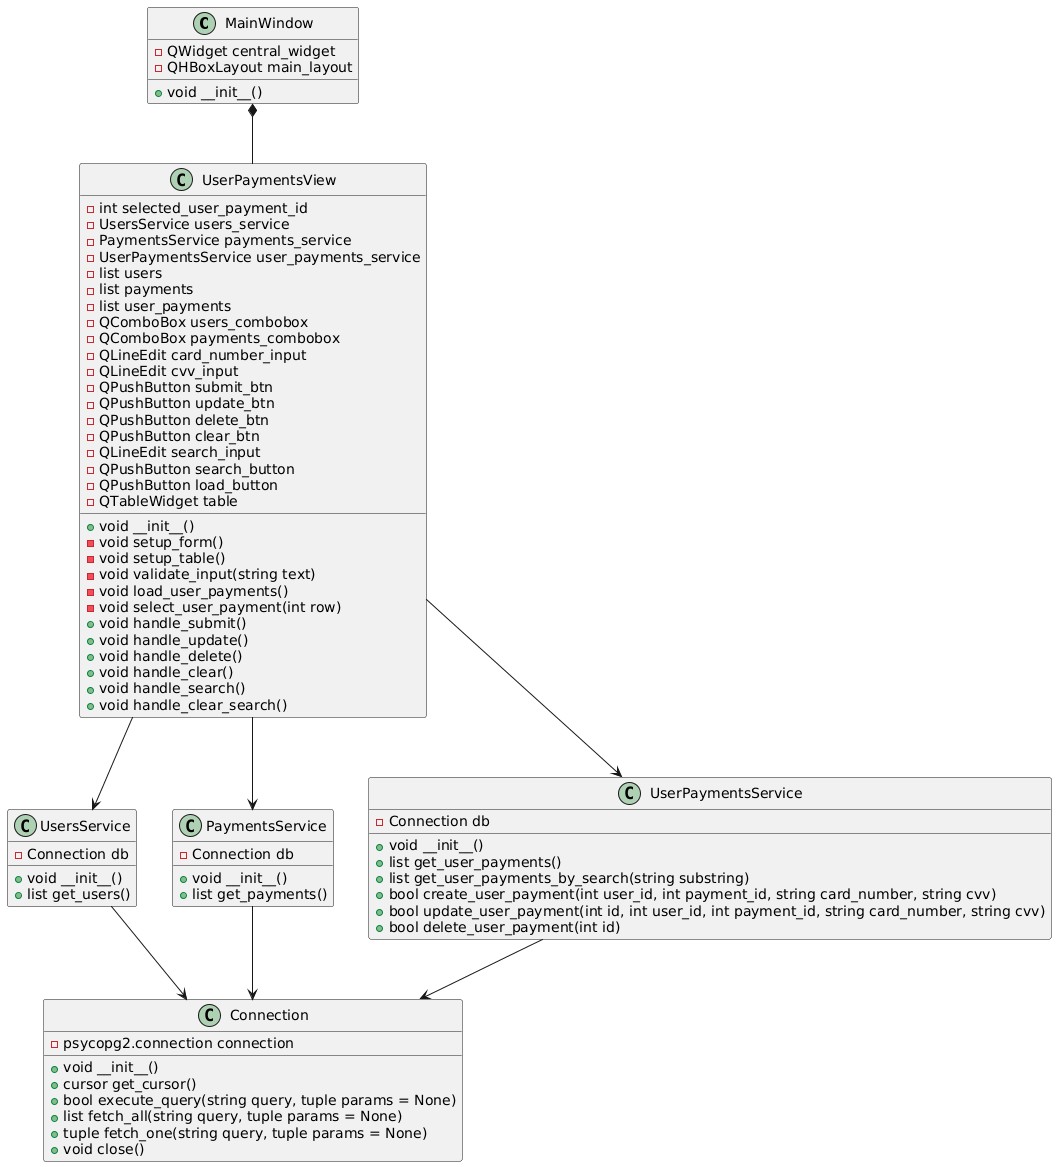
\includegraphics[width=1\linewidth]{img/uml-python.png}
  \end{figure}
  \begin{center}
    Рисунок 1 – Диаграмма классов
  \end{center}

  \pagebreak
  \begin{figure}[h]
    \centering
    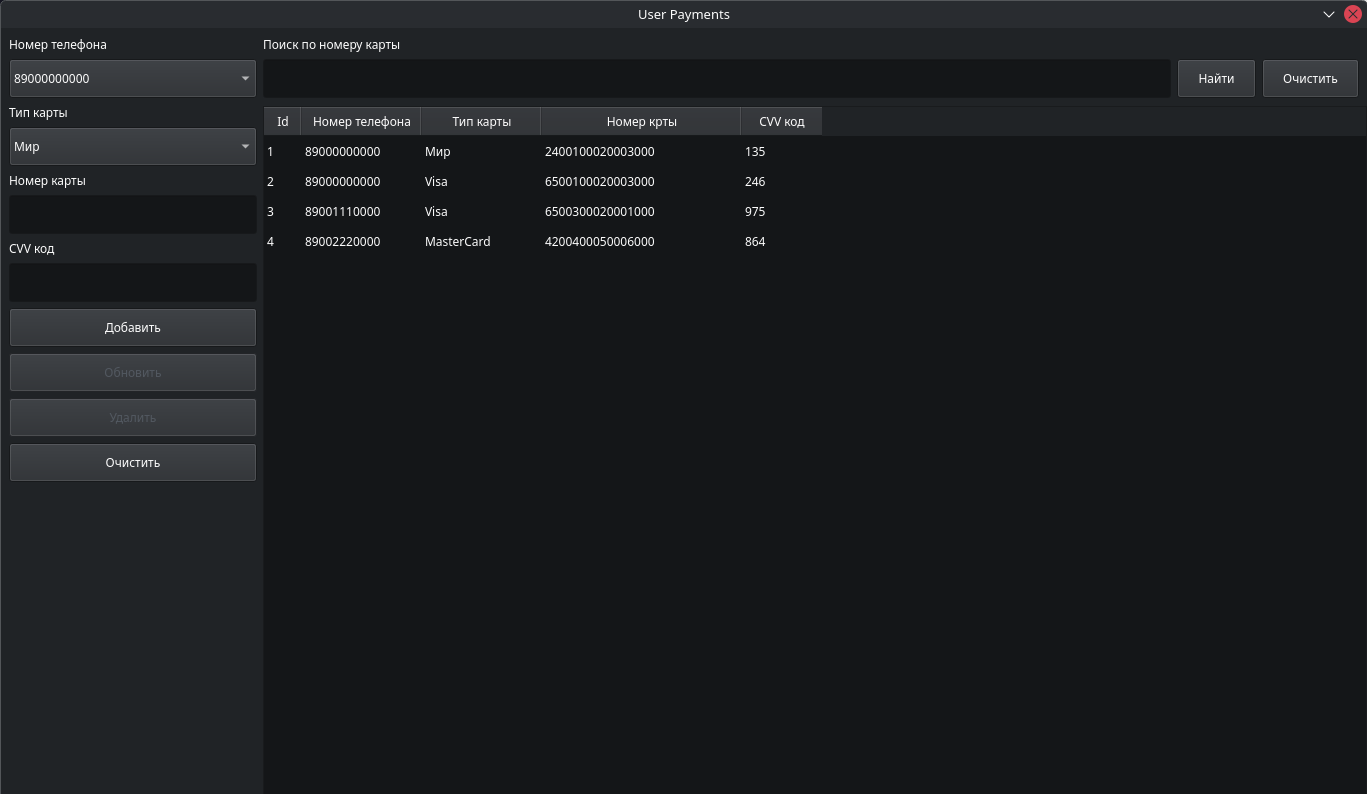
\includegraphics[width=0.95\linewidth]{img/f-1}
  \end{figure}
  \begin{center}
    Рисунок 2 – Форма таблицы способов оплаты пользователя
  \end{center}

  \begin{figure}[h]
    \centering
    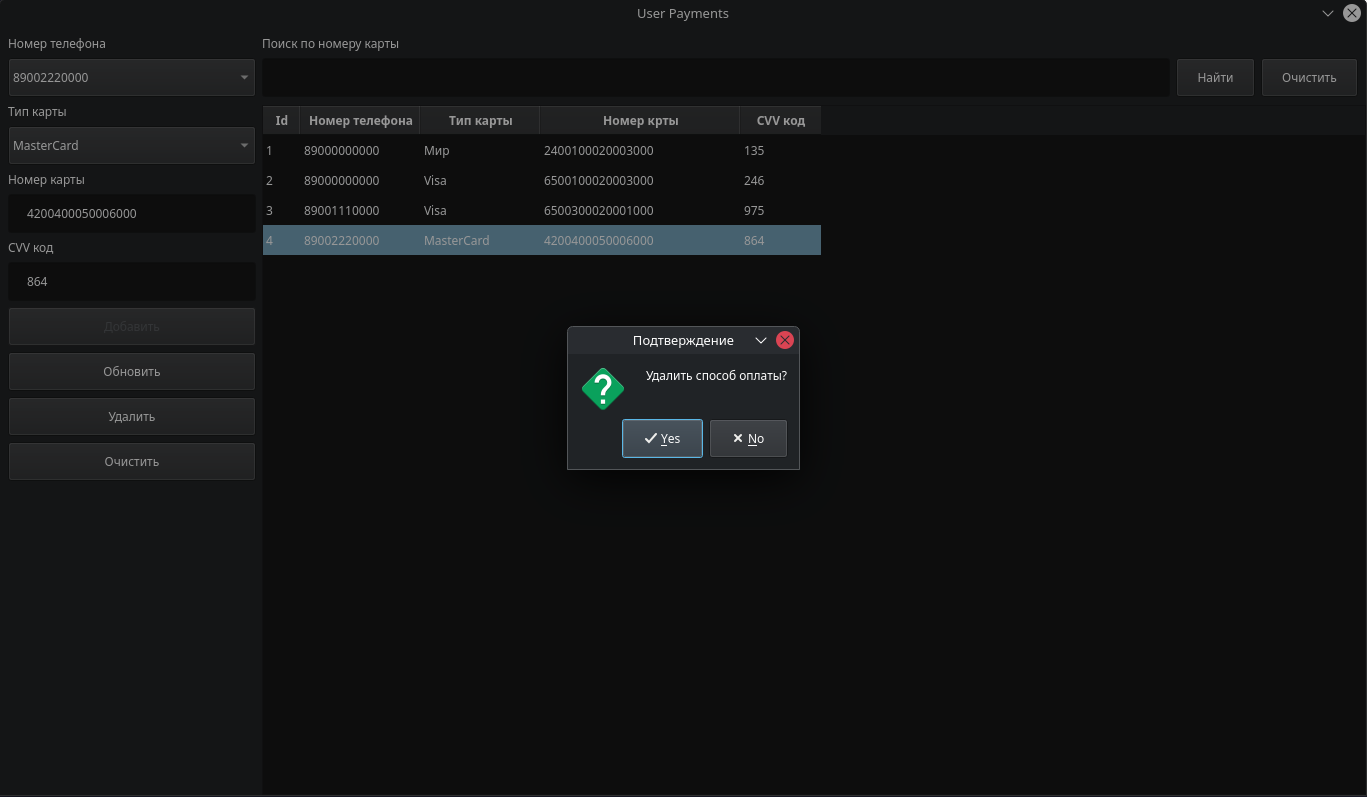
\includegraphics[width=0.95\linewidth]{img/f-2}
  \end{figure}
  \begin{center}
    Рисунок 3 – Подтверждение удаления записи
  \end{center}

  \pagebreak
  \begin{figure}[h]
    \centering
    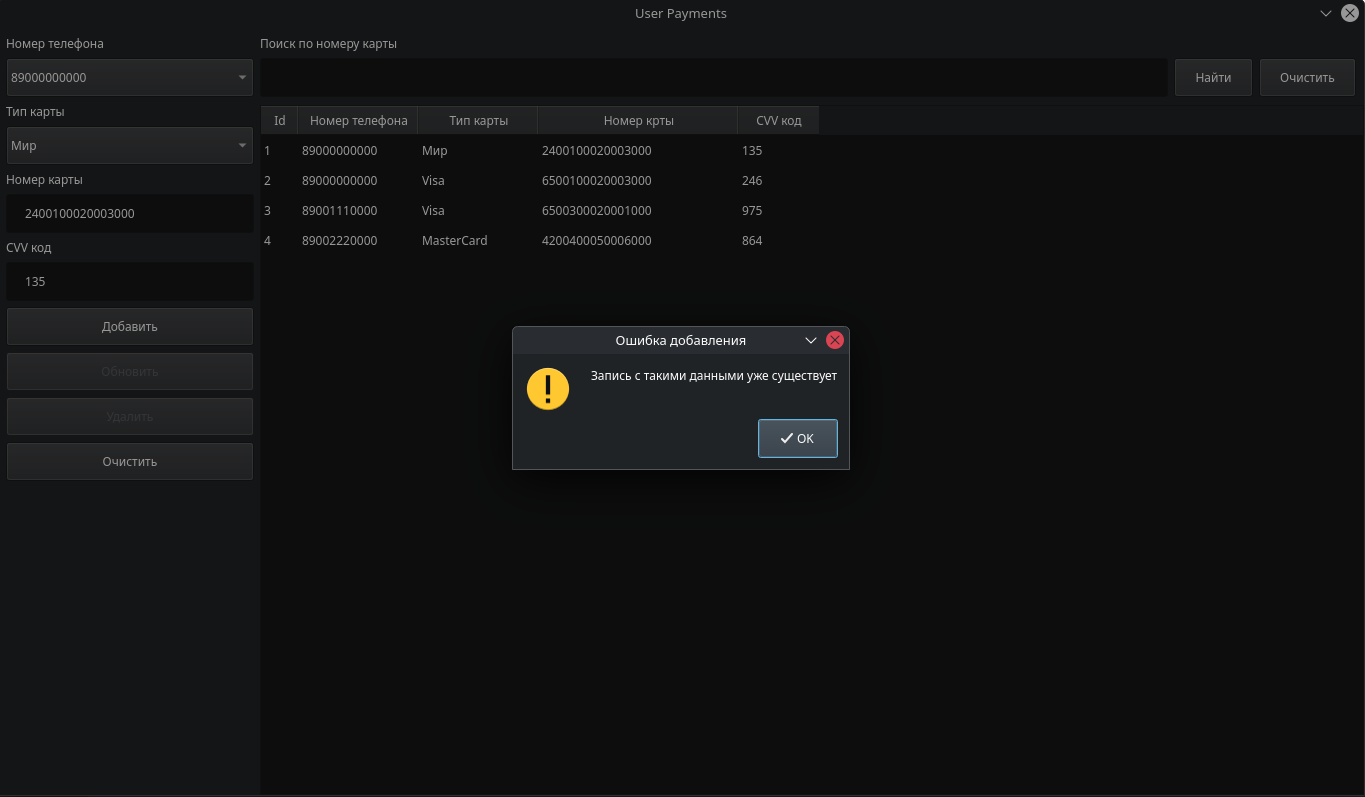
\includegraphics[width=0.95\linewidth]{img/f-3}
  \end{figure}
  \begin{center}
    Рисунок 4 – Сообщение при добавлении существующей записи
  \end{center}

  \begin{figure}[h]
    \centering
    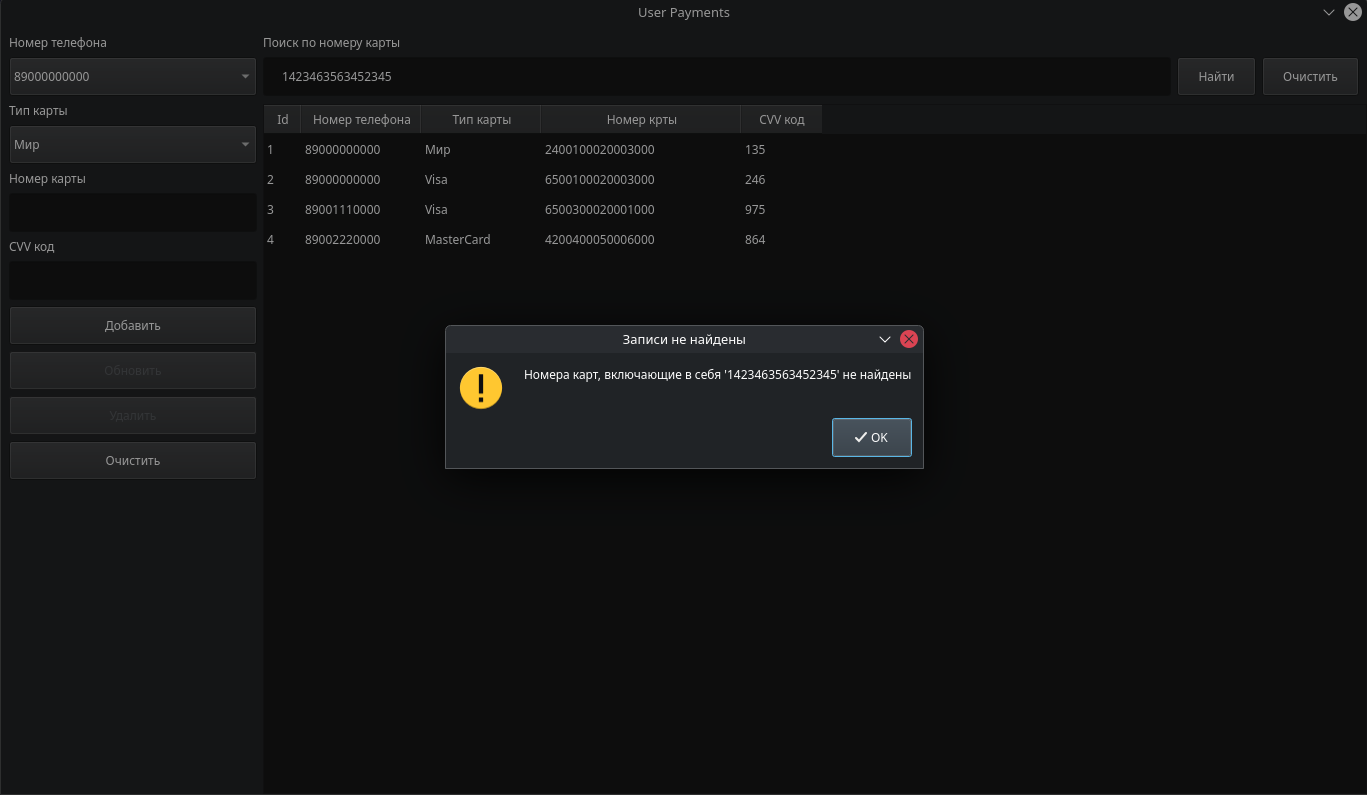
\includegraphics[width=0.95\linewidth]{img/f-4}
  \end{figure}
  \begin{center}
    Рисунок 5 – Сообщение при не найденных записях
  \end{center}

  \pagebreak
  \noindent
  \begin{Verbatim}[tabsize=4,fontsize=\small]
import sys

from PyQt6.QtWidgets import QApplication
from windows.main_window import MainWindow

def main():
    app = QApplication(sys.argv)

    window = MainWindow()
    window.show()

    sys.exit(app.exec())

if __name__ == '__main__':
    main()

import psycopg2
import psycopg2.extras

class Connection:
    connection = None

    def __init__(self):
        self.connection = psycopg2.connect(
          "dbname=dm_db user=root password=root host=localhost port=5432"
        )

    def get_cursor(self):
        return self.connection.cursor(cursor_factory=psycopg2.extras.DictCursor)
  
    def execute_query(self, query, params=None):
        cursor = self.get_cursor()
        try:
            cursor.execute(query, params)
            self.connection.commit()

            return True
        except Exception as e:
            self.connection.rollback()
            print(f"Database error: {e}")

            return False
        finally:
            cursor.close()

    def fetch_all(self, query, params=None):
        cursor = self.get_cursor()

        try:
            cursor.execute(query, params)
            results = cursor.fetchall()

            return results
        except Exception as e:
            print(f"Database error: {e}")

            return None
        finally:
            cursor.close()

    def fetch_one(self, query, params=None):
        cursor = self.get_cursor()

        try:
            cursor.execute(query, params)
            result = cursor.fetchone()

            return result
        except Exception as e:
            print(f"Database error: {e}")

            return None
        finally:
            cursor.close()

    def close(self):
        self.connection.close()

db = Connection()

from database.connection import db

class UsersService:
    def __init__(self):
        self.db = db

    def get_users(self):
        users = self.db.fetch_all("SELECT * FROM users ORDER BY id")
        if users is None:
            return []
        return users

from database.connection import db

class PaymentsService:
    def __init__(self):
        self.db = db

    def get_payments(self):
        payments = self.db.fetch_all("SELECT * FROM payments")
        if payments is None:
            return []
        return payments

from database.connection import db

class UserPaymentsService:
    def __init__(self):
        self.db = db

    def get_user_payments(self):
        payments = self.db.fetch_all(
            "SELECT up.id, u.phone_number, p.title, up.card_number, up.cvv " \
            "FROM user_payments up " \
                "JOIN users u ON u.id = up.user_id " \
                "JOIN payments p ON p.id = up.payment_id"
        )
        if payments is None:
            return []
        return payments

    def get_user_payments_by_search(self, substring):
        payments = self.db.fetch_all(
            "SELECT up.id, u.phone_number, p.title, up.card_number, up.cvv " \
                "FROM user_payments up " \
                "JOIN users u ON u.id = up.user_id " \
                "JOIN payments p ON p.id = up.payment_id " \
            f"WHERE up.card_number LIKE '%{substring}%'"
        )
        if payments is None:
            return []
        return payments

    def create_user_payment(self, user_id, payment_id, card_number, cvv):
        return self.db.execute_query(
            f"SELECT create_user_payment({user_id}, {payment_id}, '{card_number}', '{cvv}')"
        )

    def update_user_payment(self, id, user_id, payment_id, card_number, cvv):
        return self.db.execute_query(
            f"SELECT update_user_payment({id}, {user_id}, {payment_id}, '{card_number}', '{cvv}')"
        )

    def delete_user_payment(self, id):
        return self.db.execute_query(f"DELETE FROM user_payments WHERE id = {id}")

from PyQt6.QtWidgets import (
    QMainWindow, QWidget, QHBoxLayout
)
from windows.views.user_payments_view import UserPaymentsView

class MainWindow(QMainWindow):
    def __init__(self):
        super().__init__()

        central_widget = QWidget()

        main_layout = QHBoxLayout(central_widget)
        main_layout.setContentsMargins(0, 0, 0, 0)
        main_layout.addSpacing(0)
        main_layout.addWidget(UserPaymentsView())

        self.setWindowTitle("User Payments")
        self.setFixedSize(1366, 768)
        self.setCentralWidget(central_widget)

        with open('main.qss', 'r') as f:
            styles = f.read()
            self.setStyleSheet(styles)

from PyQt6.QtWidgets import (
    QWidget, QHBoxLayout, QVBoxLayout, QLineEdit, QLabel,
    QTableWidget, QTableWidgetItem, QPushButton, QMessageBox,
    QHeaderView, QComboBox
)
from PyQt6.QtCore import Qt
from services.users_service import UsersService
from services.payments_service import PaymentsService
from services.user_payments_service import UserPaymentsService

class UserPaymentsView(QWidget):
    selected_user_payment_id = None

    def __init__(self):
        super().__init__()

        self.users_service = UsersService()
        self.payments_service = PaymentsService()
        self.user_payments_service = UserPaymentsService()

        self.users = self.users_service.get_users()
        self.payments = self.payments_service.get_payments()
        self.user_payments = []

        self.main_layout = QHBoxLayout(self)
        self.main_layout.setContentsMargins(0, 0, 0, 0)

        self.setup_form()
        self.setup_table()
        self.load_user_payments()

    def setup_form(self):
        self.users_combobox = QComboBox()
        for user in self.users:
            self.users_combobox.addItem(user[1], userData=user[0])

        self.payments_combobox = QComboBox()
        for payment in self.payments:
            self.payments_combobox.addItem(payment[1], userData=payment[0])

        self.card_number_input = QLineEdit()
        self.card_number_input.setMaxLength(16)
        self.card_number_input.textChanged.connect(self.validate_input)

        self.cvv_input = QLineEdit()
        self.cvv_input.setMaxLength(3)
        self.cvv_input.textChanged.connect(self.validate_input)

        self.submit_btn = QPushButton("Добавить")
        self.submit_btn.clicked.connect(self.handle_submit)

        self.update_btn = QPushButton("Обновить")
        self.update_btn.clicked.connect(self.handle_update)
        self.update_btn.setEnabled(False)

        self.delete_btn = QPushButton("Удалить")
        self.delete_btn.clicked.connect(self.handle_delete)
        self.delete_btn.setEnabled(False)

        self.clear_btn = QPushButton("Очистить")
        self.clear_btn.clicked.connect(self.handle_clear)

        form_layout = QVBoxLayout()
        form_layout.setContentsMargins(8, 8, 0, 0)
        form_layout.setAlignment(Qt.AlignmentFlag.AlignTop)

        form_layout.addWidget(QLabel("Номер телефона"))
        form_layout.addWidget(self.users_combobox)
        form_layout.addWidget(QLabel("Тип карты"))
        form_layout.addWidget(self.payments_combobox)
        form_layout.addWidget(QLabel("Номер карты"))
        form_layout.addWidget(self.card_number_input)
        form_layout.addWidget(QLabel("CVV код"))
        form_layout.addWidget(self.cvv_input)
        form_layout.addWidget(self.submit_btn)
        form_layout.addWidget(self.update_btn)
        form_layout.addWidget(self.delete_btn)
        form_layout.addWidget(self.clear_btn)

        form_container = QWidget()
        form_container.setFixedWidth(256)
        form_container.setLayout(form_layout)

        self.main_layout.addWidget(form_container)

    def setup_table(self):
        self.search_input = QLineEdit()
        self.search_input.setMaxLength(16)
        self.search_input.textChanged.connect(self.validate_input)

        self.search_button = QPushButton("Найти")
        self.search_button.clicked.connect(self.handle_search)

        self.load_button = QPushButton("Очистить")
        self.load_button.clicked.connect(self.handle_clear_search)

        self.table = QTableWidget()
        self.table.setColumnCount(5)
        self.table.verticalHeader().setVisible(False)
        self.table.setHorizontalHeaderLabels(
          ["Id", "Номер телефона", "Тип карты", 
            "Номер крты", "CVV код"]
        )
        self.table.setColumnWidth(0, 20)
        self.table.setColumnWidth(1, 120)
        self.table.setColumnWidth(2, 120)
        self.table.setColumnWidth(3, 200)
        self.table.setColumnWidth(4, 80)
        self.table.cellClicked.connect(self.select_user_payment)
        self.table.setShowGrid(False)

        self.table.horizontalHeader()
          .setSectionResizeMode(0, QHeaderView.ResizeMode.Fixed)
        self.table.horizontalHeader()
          .setSectionResizeMode(1, QHeaderView.ResizeMode.Fixed)
        self.table.horizontalHeader()
          .setSectionResizeMode(2, QHeaderView.ResizeMode.Fixed)
        self.table.horizontalHeader()
          .setSectionResizeMode(3, QHeaderView.ResizeMode.Fixed)
        self.table.horizontalHeader()
          .setSectionResizeMode(4, QHeaderView.ResizeMode.Fixed)
        self.table.setSelectionBehavior(
          QTableWidget.SelectionBehavior.SelectRows
        )

        search_layout = QVBoxLayout()
        search_layout.setContentsMargins(0, 8, 8, 8)

        search_input_layout = QHBoxLayout()
        search_input_layout.setContentsMargins(0, 0, 0, 0)

        search_input_layout.addWidget(self.search_input)
        search_input_layout.addWidget(self.search_button)
        search_input_layout.addWidget(self.load_button)

        search_layout.addWidget(QLabel("Поиск по номеру карты"))
        search_layout.addLayout(search_input_layout)

        search_container = QWidget()
        search_container.setLayout(search_layout)

        table_layout = QVBoxLayout()
        table_layout.setContentsMargins(0, 0, 0, 0)
        table_layout.setSpacing(0)

        table_layout.addWidget(search_container)
        table_layout.addWidget(self.table)

        main_container = QWidget()
        main_container.setLayout(table_layout)

        self.main_layout.addWidget(main_container)

    def validate_input(self, text):
        if text and not text.isdigit():
            self.sender().setText(text[:-1])
            QMessageBox.warning(self, "Ошибка ввода", "Разрешены только цифры")

    def load_user_payments(self):
        self.user_payments = self.user_payments_service.get_user_payments()

        self.table.setRowCount(len(self.user_payments))

        for row, user in enumerate(self.user_payments):
            self.table.setItem(row, 0, QTableWidgetItem(str(user[0])))
            self.table.setItem(row, 1, QTableWidgetItem(str(user[1])))
            self.table.setItem(row, 2, QTableWidgetItem(str(user[2])))
            self.table.setItem(row, 3, QTableWidgetItem(str(user[3])))
            self.table.setItem(row, 4, QTableWidgetItem(str(user[4])))

    def select_user_payment(self, row):
        item_id = self.table.item(row, 0)
        if item_id:
            self.selected_user_payment_id = int(item_id.text())

            phone_number_item = self.table.item(row, 1)
            payment_item = self.table.item(row, 2)
            card_number_item = self.table.item(row, 3)
            cvv_item = self.table.item(row, 4)

            phone_number_index = self.users_combobox.findText(
              phone_number_item.text()
            )
            payment_index = self.payments_combobox.findText(
              payment_item.text()
            )

            if phone_number_item:
                self.users_combobox.setCurrentIndex(phone_number_index)
            if phone_number_item:
                self.payments_combobox.setCurrentIndex(payment_index)
            if card_number_item:
                self.card_number_input.setText(card_number_item.text())
            if cvv_item:
                self.cvv_input.setText(cvv_item.text())

            self.update_btn.setEnabled(True)
            self.delete_btn.setEnabled(True)
            self.submit_btn.setEnabled(False)

    def handle_submit(self):
        user_id = self.users_combobox.currentData()
        payment_id = self.payments_combobox.currentData()
        card_number = self.card_number_input.text()
        cvv = self.cvv_input.text()

        if not card_number or not cvv:
            QMessageBox.warning(self,
              "Ошибка", "Все поля обязательны для заполнения"
            )
            return

        for card in self.user_payments:
            if card['card_number'] == card_number:
                QMessageBox.warning(self, "Ошибка добавления",
                  "Запись с такими данными уже существует"
                )
                return

        self.user_payments_service.create_user_payment(
          user_id, payment_id, card_number, cvv
        )
        self.handle_clear()
        self.load_user_payments()

    def handle_update(self):
        if self.selected_user_payment_id is None:
            return

        user_id = self.users_combobox.currentData()
        payment_id = self.payments_combobox.currentData()
        card_number = self.card_number_input.text()
        cvv = self.cvv_input.text()

        if not card_number or not cvv:
            QMessageBox.warning(self, "Ошибка", 
              "Все поля обязательны для заполнения"
            )
            return

        self.user_payments_service.update_user_payment(
          self.selected_user_payment_id, user_id, payment_id, card_number, cvv
        )
        self.handle_clear()
        self.load_user_payments()

    def handle_delete(self):
        if self.selected_user_payment_id is None:
            return

        reply = QMessageBox.question(
            self,
            "Подтверждение",
            "Удалить способ оплаты?",
            QMessageBox.StandardButton.Yes | QMessageBox.StandardButton.No
        )

        if reply == QMessageBox.StandardButton.Yes:
            self.user_payments_service.delete_user_payment(
              self.selected_user_payment_id
            )
            self.handle_clear()
            self.load_user_payments()

    def handle_clear(self):
        self.users_combobox.setCurrentIndex(0)
        self.payments_combobox.setCurrentIndex(0)
        self.card_number_input.clear()
        self.cvv_input.clear()
        self.selected_user_payment_id = None
        self.submit_btn.setEnabled(True)
        self.update_btn.setEnabled(False)
        self.delete_btn.setEnabled(False)
        self.table.clearSelection()

    def handle_search(self):
        search = self.search_input.text().strip()

        if not search:
            QMessageBox.warning(self, 
              "Ошибка", "Поле поиска обязательно для заполнения"
            )
            return

        user_payments = 
          self.user_payments_service.get_user_payments_by_search(search)

        if (len(user_payments) == 0):
            QMessageBox.warning(self, "Записи не найдены", 
              f"Номера карт, включающие в себя '{search}' не найдены"
            )
            return

        self.table.setRowCount(len(user_payments))

        for row, user in enumerate(user_payments):
            self.table.setItem(row, 0, QTableWidgetItem(str(user[0])))
            self.table.setItem(row, 1, QTableWidgetItem(str(user[1])))
            self.table.setItem(row, 2, QTableWidgetItem(str(user[2])))
            self.table.setItem(row, 3, QTableWidgetItem(str(user[3])))
            self.table.setItem(row, 4, QTableWidgetItem(str(user[4])))

    def handle_clear_search(self):
        self.search_input.clear()
        self.load_user_payments()
  \end{Verbatim}

  \section*{Вывод}
  В ходе выполнения лабораторной работы освоили библиотеки Python для связывания с БД, разработоно классическое десктопное приложение для управления данными в таблице способов оплаты пользователя.

\end{document}